% !TEX root = Projektdokumentation.tex
\section{Anhang}
\label{sec:Anhang}
\subsection{Gantt-Diagramm und Meilensteine}
\label{app:Gantt}
\includegraphicsKeepAspectRatio{Anhang/Gantt.pdf}{1}
\clearpage

\subsection{Detaillierte Zeitplanung}
\label{app:Zeitplanung}
\tabelleAnhang{ZeitplanungKomplett}
\clearpage

\subsection{Use Case-Diagramm}
\label{app:UseCase}
\begin{figure}[htb]
\centering
\includegraphicsKeepAspectRatio{Anhang/UseCaseCloudInfra.png}{1}
\caption{Use Case-Diagramm}
\end{figure}
\clearpage

\subsection{Sequenzdiagramm CLI Zugriff auf die Instanzen}
\label{app:Sequenzdiagramm CLI Zugriff auf die Instanzen}
\includegraphicsKeepAspectRatio{Anhang/SequenzDiagrammCLI.png}{1}
\clearpage

\subsection{Cloud-Infrastruktur}
\label{app:Cloud-Infrastruktur}
\begin{figure}[htb]
    \centering
    \includegraphicsKeepAspectRatio{Anhang/Cloud-Infra-Topology.png}{1}
\end{figure}
\pagebreak

\subsection{docker-compose.yml}
\label{app:docker-compose.yml}
\includegraphicsKeepAspectRatio{Anhang/docker-compose.pdf}{0.9}

\subsection{.env}
\label{app:dotenv}
\includegraphicsKeepAspectRatio{Anhang/(.)env.pdf}{0.9}

\subsection{Docker-Befehle}
\label{app:dockercommands}
\begin{figure}[ht]
    \centering
    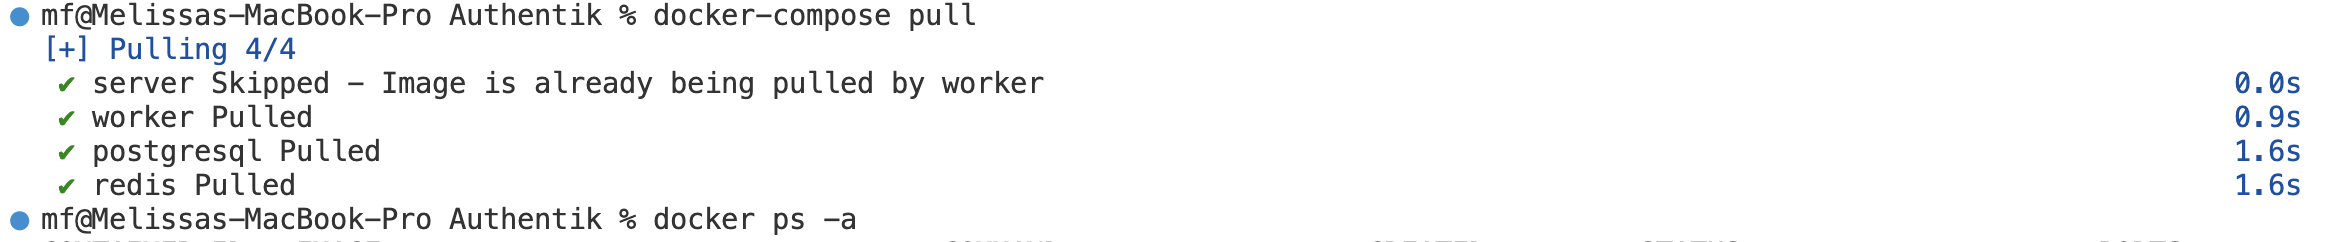
\includegraphics[scale=0.4]{Bilder/Authentik-Doc/DP_00_DockerPull.png}
    \caption{Docker Pull}
  \end{figure}
  
  \vspace{0.5cm} % Adjust vertical space as needed
  
  \begin{figure}[ht]
    \centering
    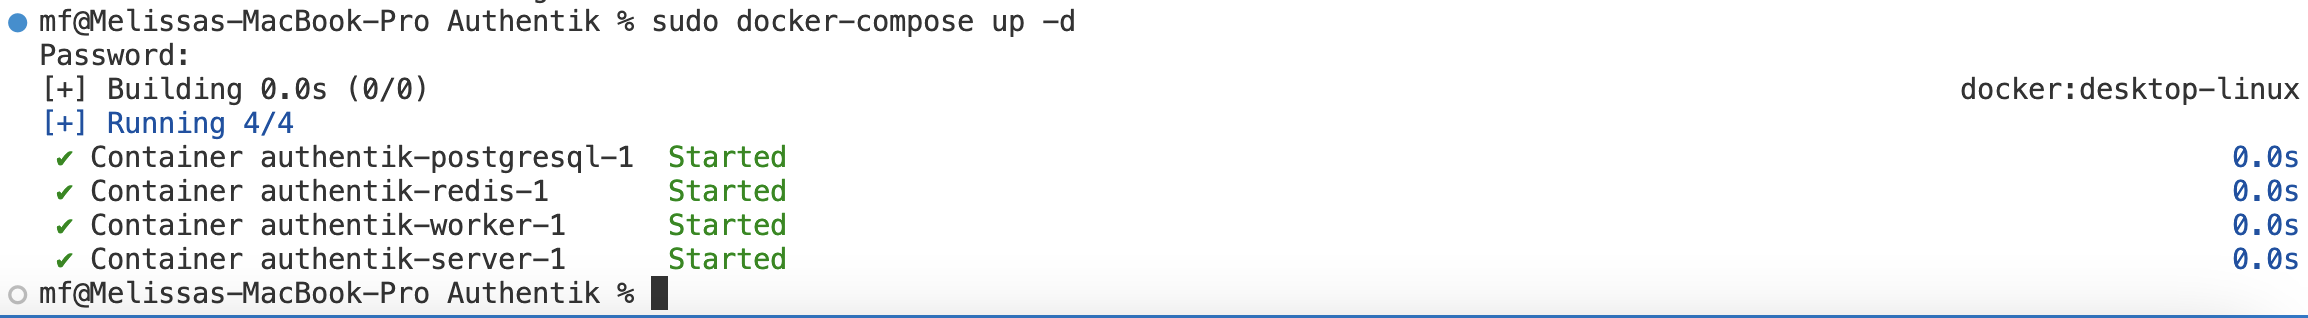
\includegraphics[scale=0.4]{Bilder/Authentik-Doc/DP_01_DockerComposeUp.png}
    \caption{Docker Compose Up}
  \end{figure}

\subsection{Proxy Host Konfiguration}
\label{app:ProxyHostConfig}
\includegraphicsKeepAspectRatio{Anhang/ProxyHostKonfiguration.pdf}{0.9}

\subsection{Authentik-Konfiguration}
\label{app:AuthentikConfig}
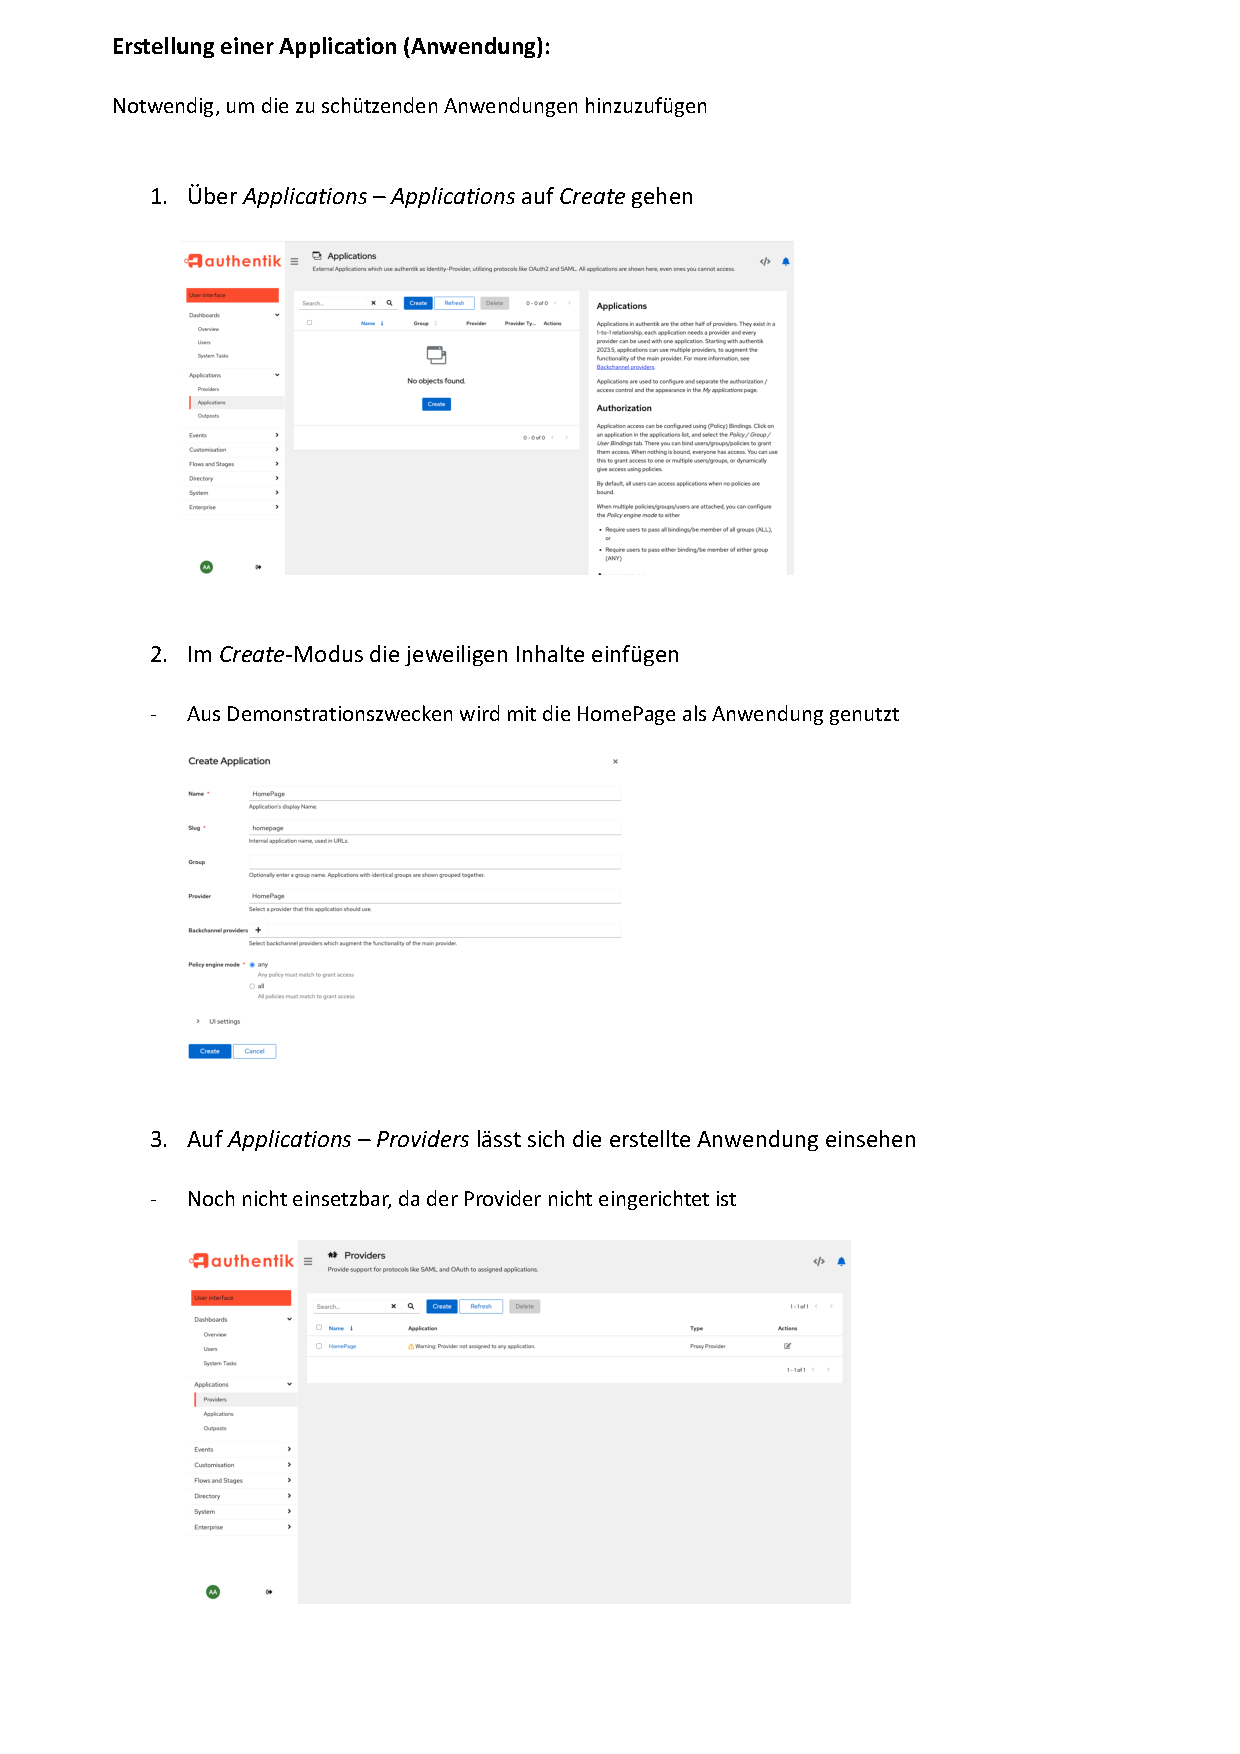
\includepdf[pages={1-3}, scale=0.9]{Anhang/Authentik-Konfiguration.pdf}

\subsection{NGinx Konfiguration}
\label{app:CustomNGinxConfig}
\includegraphicsKeepAspectRatio{Anhang/Custom_NGinx_Configuration.pdf}{0.9}
\clearpage
\begin{figure}[htb]
    \centering
    \includegraphicsKeepAspectRatio{Bilder/Authentik-Doc/NS_03_ChangeIPInCustomNGinxConfig.png}{0.4}
    \captionbelow{Proxy Host Konfiguration - Einfügen des Code-Snippets in den Bereich \textbf{Advanced} 
    und erfolgt das Ändern der IP-Adresse mit dem zugehörigen Port}
\end{figure}

\subsection{TOTP-Einrichtung}
\label{sec:TOTPConfig}
\includegraphicsKeepAspectRatio{Anhang/TOTP-Einrichtung.pdf}{0.9}

\subsection{Benutzerdokumentation}
\label{app:Benutzerdokumentation}
\includegraphicsKeepAspectRatio{Anhang/Benutzerdokumentation.pdf}{0.9}